Stars are thermonuclear structures held in balance by a competition between gravitational contraction and internal pressure. This pressure arises from nuclear fusion: the conversion of light elements into heavier ones, accompanied by energy release. The dominant fusion pathway depends on stellar mass. In relatively low-mass stars, such as the Sun, hydrogen is fused into helium primarily through a sequence of reactions called the proton-proton chain. In more massive stars, the dominant process is the carbon–nitrogen–oxygen (CNO) cycle, in which hydrogen nuclei fuse into helium via catalytic reactions involving heavier nuclei. The CNO cycle requires higher temperatures and therefore occurs only in hotter stellar cores.

Stellar evolution proceeds as nuclear fuel is gradually exhausted. Once hydrogen fusion subsides, gravity compresses the core, raising the temperature and enabling new fusion stages. Helium is converted into carbon and oxygen, followed by carbon, neon, oxygen, and silicon burning in increasingly rapid succession. These stages produce progressively heavier elements, up to iron. Fusion beyond iron is endothermic, and no further energy can be extracted from nuclear reactions.

The fate of a star is determined primarily by its initial mass. Stars with initial masses below approximately eight times that of the Sun — less than about $8$ solar masses — do not reach the conditions needed for heavy-element fusion. Their cores contract into white dwarfs composed of carbon and oxygen, while their outer layers are ejected as planetary nebulae. White dwarfs are stabilized by electron degeneracy pressure, which can support them only up to a critical mass known as the Chandrasekhar limit, roughly $1.4$ times the Sun's mass.

Heavier stars proceed through all stages of nuclear burning, eventually developing iron cores. As no further fusion is energetically favorable, the core becomes dynamically unstable and collapses in milliseconds. Infalling material rebounds off the dense core and triggers a violent explosion that ejects the outer layers. This core-collapse supernova leaves behind a neutron star or, if massive enough, a black hole.

Supernovae are classified according to their spectral features. Type II supernovae retain strong hydrogen lines and arise from stars that preserve their outer hydrogen envelopes. Type Ib and Ic supernovae lack hydrogen and, in the latter case, helium signatures, indicating extensive pre-explosion mass loss. These core-collapse events produce irregular light curves and depend sensitively on progenitor structure.

Type Ia supernovae originate from a different mechanism. These events occur when a white dwarf in a binary system accretes matter from a companion and approaches the Chandrasekhar mass. Internal pressure can no longer counteract gravity, and carbon and oxygen ignite under degenerate conditions in a runaway thermonuclear reaction. The white dwarf is completely disrupted, releasing a sharply peaked and reproducible amount of energy. Unlike core-collapse events, Type Ia supernovae leave no remnant. Their uniformity leads to a characteristic light curve with a distinctive rise and decay pattern, allowing for empirical standardization and making them powerful cosmological distance indicators.

In observational cosmology, Type Ia supernovae serve as standard candles: sources whose intrinsic luminosity $L$ can be inferred with relatively low scatter after empirical correction. When such an object is observed, its apparent flux $F$ — the energy received per unit area per unit time — is measured at Earth. Under the assumption that the source radiates isotropically in flat space, flux and luminosity are related by the inverse-square law:$F = \frac{L}{4\pi d_L^2}, $ where $d_L$ is the luminosity distance. This expression defines $d_L$ as the hypothetical distance at which the source would produce the observed flux if space were Euclidean and transparent.

In practice, rather than quoting $F$ directly, astronomers use a logarithmic brightness scale based on magnitudes. The apparent magnitude $m$ is a logarithmic measure of $F$, while the absolute magnitude $M$ corresponds to the magnitude the source would have at a standard distance of 10 parsecs. Their difference defines the distance modulus:
\[
\mu = m - M = 5 \log_{10}\left( \frac{d_L}{\text{Mpc}} \right) + 25.
\]
This formulation accommodates both historical conventions and the logarithmic sensitivity of human vision. For Type Ia supernovae, $M$ is not strictly constant, but correlates with the light curve shape — brighter events fade more slowly. After correcting for this effect and for color-dependent extinction, the remaining scatter in standardized magnitudes is sufficiently small to extract cosmological information.

Each supernova provides two observables: a redshift $z$ and a distance modulus $\mu(z)$. The redshift is defined by
\[
1 + z = \frac{\lambda_{\text{obs}}}{\lambda_{\text{emit}}},
\]
where $\lambda_{\text{emit}}$ is the rest-frame emission wavelength and $\lambda_{\text{obs}}$ is the observed wavelength. At low redshift, this corresponds to a Doppler shift, but at cosmological scales it reflects changes in the scale factor of the universe. The set of points $(z, \mu)$ defines a Hubble diagram, which encodes the history of cosmic expansion.

In the 1990s, two major collaborations — the Supernova Cosmology Project and the High-Z Supernova Search Team — used wide-field imaging and rapid spectroscopic follow-up to discover and monitor Type Ia supernovae out to redshifts near $z \sim 1$. These campaigns required coordinated use of ground-based telescopes and, in key cases, the Hubble Space Telescope. Each confirmed event was monitored across multiple bands over time, and light curves were compared to empirical templates. Corrections for interstellar extinction and host-galaxy properties were applied to refine the inferred luminosity.

The data showed that distant supernovae were consistently fainter than expected for a decelerating universe. The effect appeared across filters, instruments, and reduction methods. It was not eliminated by correcting for observational selection or intrinsic variation. Cross-calibration against low-redshift samples and repeated observations supported the result. The implication was that the universe had expanded more during the photon's travel time than would occur under gravitational deceleration alone. This requires that the expansion rate was increasing over time.

In cosmology, the large-scale evolution of the universe is described by a time-dependent scale factor $a(t)$, which determines how proper distances between comoving points change with cosmic time. A monotonically increasing $a(t)$ corresponds to expansion, while the behavior of its second derivative distinguishes decelerating from accelerating regimes. Acceleration occurs when $\ddot{a}(t) > 0, $ indicating that the rate of expansion is itself increasing. This cannot be produced by matter or radiation alone — both contribute positive energy density and non-negative pressure, which lead to deceleration under the Einstein field equations. A component with sufficiently negative pressure must dominate the energy content to reverse this trend. Supernova observations revealed this directly: the luminosity distance $d_L(z)$, inferred from apparent brightness and calibrated absolute magnitude, increases more rapidly with redshift than would be expected in a decelerating universe. No model-dependent priors were required — the conclusion followed from the empirical relation between redshift and distance.

Further support came from measurements of the cosmic microwave background. The angular structure of the temperature fluctuations indicates that spatial geometry is nearly flat. Yet, the matter density — ordinary and dark combined — accounts for only about a third of the required energy density for flatness. The remaining contribution must come from a non-clustering, smooth component. Observations of large-scale structure, including the imprint of baryon acoustic oscillations, are consistent with this picture. The evolution of structure on cosmic scales also reflects the influence of accelerated expansion.

The coherence of these observational lines led to rapid adoption of the acceleration result. No single dataset is sufficient, but their joint consistency across methods and scales leaves little room for alternatives. Type Ia supernovae first detected the effect. Microwave background and structure surveys confirmed its implications.

The possibility of a component that modifies expansion on large scales had been considered decades earlier. In 1917, Einstein added a constant term $\Lambda$ to the relativistic field equations to construct a static cosmological model. At the time, the known universe showed no evidence of motion on the largest scales. The cosmological constant introduced a uniform repulsive influence that balanced gravity exactly. This static solution was unstable and soon discarded after Hubble's 1929 observations demonstrated that galaxies are receding from one another. The cosmological constant was removed from most models and became a historical footnote.

Its mathematical form, however, remained valid. $\Lambda$ represents a constant energy density that does not dilute as the universe expands. In general relativity, it enters the dynamics with a sign and magnitude that oppose the deceleration caused by matter. In quantum field theory, the vacuum itself carries an energy density that enters the gravitational field equations with the same formal structure. Estimates of this vacuum energy, however, exceed observed values by many orders of magnitude, creating a mismatch that remains unresolved.

When supernova observations revealed that expansion is accelerating, the cosmological constant returned — not to restore symmetry, but to match data. Its inclusion in the equations adjusts the predicted luminosity-distance curve in a way that aligns with the observations. This reappearance was not a theoretical preference, but a response to a measured deviation in the Hubble diagram.

The term "dark energy" refers to whatever component drives the observed acceleration of cosmic expansion. It denotes a form of energy whose dynamical behavior differs fundamentally from that of matter or radiation. Dark energy does not cluster on small scales, and its energy density remains nearly constant — or even increases — as the universe expands. In its simplest form, it corresponds to a constant vacuum energy density $\Lambda$. More general frameworks allow this component to vary with time. Theoretical models typically describe dark energy either as a scalar field whose potential energy dominates its evolution, producing negative pressure, or as a modification of general relativity in which the gravitational field equations are altered to permit acceleration without introducing exotic matter.

What defines dark energy observationally is its role in producing accelerated expansion. Models that exclude it fail to match the supernova Hubble diagram, the angular structure of the microwave background, and the measured scale of clustering. A smooth, repulsive component is required to account for the current expansion history.

The inference of cosmic acceleration relies on direct measurement of distance and redshift. For each Type Ia supernova, a light curve is constructed from multi-band photometric observations. After correcting for light curve shape, color, and host-galaxy properties, the standardized peak magnitude serves as a proxy for intrinsic luminosity. Comparing this with observed flux yields the distance modulus $\mu$, and thus the luminosity distance $d_L$.

Redshift $z$ is measured spectroscopically by comparing observed and rest-frame wavelengths of spectral lines. Each supernova thus provides a data point $(z, \mu)$ on the Hubble diagram. In a decelerating universe, $d_L(z)$ grows more slowly than observed. The consistent excess brightness attenuation at high redshift implies that expansion has accelerated during the photon's travel time.

To rule out confounding factors such as dust extinction, progenitor evolution, or selection bias, surveys include extensive control samples at low redshift. Calibration is anchored using Cepheid variables and surface brightness fluctuations. Observational consistency is checked across telescopes, filters, and reduction pipelines.

Large-scale surveys including SNLS, SDSS-II, and the Dark Energy Survey have compiled thousands of supernovae extending to $z \sim 1.5$. Fitting these data to cosmological models yields a statistically significant preference for late-time acceleration. The observed curvature of the Hubble diagram cannot be replicated by any matter-only model.

Independent evidence supports this conclusion. Measurements of the cosmic microwave background constrain the angular diameter distance to recombination, requiring flat spatial geometry if interpreted within general relativity. Yet the matter density inferred from clustering accounts for only one-third of the critical density. Baryon acoustic oscillations further fix the expansion history by serving as a standard ruler across redshift.

The combined data constrain not only the presence of accelerated expansion, but also its detailed evolution. Future surveys — including the Vera Rubin LSST and the Roman Space Telescope — aim to refine measurements of $d_L(z)$ to sub-percent precision, distinguishing between a true cosmological constant and time-varying models of dark energy.

The acceleration of the universe is a measured phenomenon. The need for a new term in the energy budget is not speculative. It follows from the observed relation between redshift and brightness in distant stellar explosions, confirmed across independent data streams. The term "dark energy" describes this requirement. Its interpretation remains open, but its necessity is empirical.

The cosmological constant $\Lambda$ provides the simplest model for dark energy. Within general relativity, the dynamics of cosmic expansion are governed by the Friedmann equations, which describe how the scale factor $a(t)$ evolves with time. The scale factor quantifies the expansion of space itself: if two galaxies are separated by a fixed comoving distance, their physical separation increases as $a(t)$ grows.

The key insight is that acceleration depends not only on energy density but also on pressure. For ordinary matter and radiation, which exert non-negative pressure, gravity acts to decelerate the expansion. However, a component with sufficiently negative pressure can drive acceleration. The cosmological constant corresponds to a uniform energy density that exerts negative pressure equal to its energy density. This negative pressure acts as a repulsive gravitational source, causing space itself to expand at an accelerating rate.

The resulting model, known as $\Lambda$CDM, successfully describes a wide range of observations. Current measurements indicate the universe is composed of approximately 68\% dark energy, 27\% dark matter, and 5\% ordinary matter. This composition explains not only the supernova observations but also the patterns observed in the cosmic microwave background and large-scale structure.

High-redshift supernovae confirm a transition from an earlier decelerating phase, when matter dominated the energy budget, to the current accelerating phase driven by dark energy. This transition occurred roughly when the universe was half its current age, when the energy densities of matter and dark energy became comparable.

Despite this empirical success, the physical nature of dark energy remains profoundly mysterious. The observed value of the cosmological constant is extraordinarily small compared to theoretical expectations from quantum field theory. Quantum mechanics predicts that even empty space should possess a vacuum energy density, arising from zero-point fluctuations of all possible fields. Yet this predicted vacuum energy exceeds the observed dark energy density by approximately 120 orders of magnitude — a discrepancy so severe it has been called "the worst theoretical prediction in the history of physics."

This cosmological constant problem exposes a fundamental gap in our understanding of quantum gravity and the structure of spacetime. Unlike other areas of physics, where only energy differences matter, general relativity couples directly to the absolute value of the energy density. The vacuum energy cannot simply be subtracted away without affecting the geometry of space and time. The resolution may require entirely new physics beyond the Standard Model or a fundamental revision of our understanding of gravity itself.

\begin{commentary}[How Much Can Be Measured]
Scientific understanding is constrained by what can be observed. In cosmology, measurements rely on electromagnetic radiation, primarily in a few accessible bands of the spectrum. Telescopes capture only a fraction of the sky at any given time. Most stars, galaxies, and intergalactic matter are never directly observed, and yet, from this limited sample, consistent physical laws have been extracted.

This is a serendipitous outcome! Sampling 0.0\ldots01\% of the universe's contents has been sufficient to uncover mathematical relationships that describe its large-scale behavior. The same formalism that governs an apple's descent also predicts planetary motion, galaxy trajectories, and the expansion of space.

The precision is remarkable: measuring a falling spoon on Earth can predict planetary orbits in distant galaxies with 99\% accuracy. Adding the considerable effort of developing and testing general relativity gains the remaining 0.99\% precision needed for GPS satellites and gravitational wave detectors. Yet despite this extraordinary success in describing gravity and motion across cosmic scales, 95\% of the total energy density in the universe remains completely unaccounted for!

Dark matter and dark energy dominate the dynamics, yet their nature is unknown. The success of mathematical modeling in organizing what is accessible illustrates both the remarkable reach of inference from incomplete information and the humbling limits of our cosmic perspective.

\end{commentary}

\newpage
\thispagestyle{empty}

\begin{center}
\vspace*{1cm}
{\Large\textbf{A Short Story}}\\[0.5cm]
{\large\textit{The Custodians of One}}
\vspace{0.5cm}
\end{center}

\begin{tcolorbox}[colback=gray!5,colframe=gray!40,boxrule=0.5pt,arc=3pt,boxsep=10pt,left=8pt,right=8pt,top=8pt,bottom=8pt]

The monastery on Tethra-9 had no name, it needed none. It was carved from igneous glass in the crust of a moon whose atmosphere had boiled off in the Proxima Flare. Inside, monks who had transcended the need for insignia, watching the null-entropy of eternity with infinite patience.

\medskip

Commander Rafe Lin arrived in \emph{Shibboleth}, a vacuum-energy cruiser whose drive core extracted work from the vacuum ground state itself. Its hull was reinforced against gradients that could collapse neutron stars into geometric points. It was an abomination, even to those who built it.

\medskip

The monks observed his approach with studied indifference. Seven levels down through recursive dimensional barriers, they found \emph{it}: a featureless black sphere hovering in defiance of every conservation law except the one that mattered.

\medskip

It was the Monad. A magnetic monopole — not merely a particle, but the \emph{arithmetic} upon which particle physics balanced its ledgers. Without it, electric charge would be as arbitrary as poetry. The gauge symmetries would unravel like a bad proof.

\medskip

"Extraction protocol, immediate," Rafe commanded, his voice carrying the authority of those who mistake correlation for causation.

\medskip

The eldest monk spoke with the gentleness reserved for those about to discover the difference between locally and globally defined: "Commander, your vessel maintains structural integrity only because spacetime agrees to be continuous. Remove the boundary condition, and agreement becomes... negotiable."

\medskip

The containment field collapsed. The sphere shifted — not through the usual four dimensions, but through the space of \emph{definitions} themselves. Somewhere, the Riemann hypothesis lost a prime. The fundamental constants performed a probabilistic quadrille.

\medskip

\emph{Shibboleth} discovered that its existence had been predicated on several no-longer-valid assumptions. The ship lost coherence with the dignity of a well-posed problem becoming suddenly ill-defined. Rafe learned, too late, that identity is a function of continuity.


\medskip

The monks reactivated containment with the practiced efficiency of librarians re-shelving infinity. The sphere returned to its fixed point. The universe exhaled. No rescue missions were authorized, for there was nothing left to rescue but mathematics.

\medskip

And the cosmos, whole once more, continued its stately rotation, because
\[
\oint_{\partial \Sigma} \mathbf{E} \cdot d\mathbf{l} = -\frac{d}{dt} \int_{\Sigma} \mathbf{B} \cdot d\mathbf{A}
\]
only holds if $\nabla \cdot \mathbf{B} \ne 0$ \emph{somewhere.}

\end{tcolorbox}

\thispagestyle{empty}
\begin{figure}[p]
\centering
\fbox{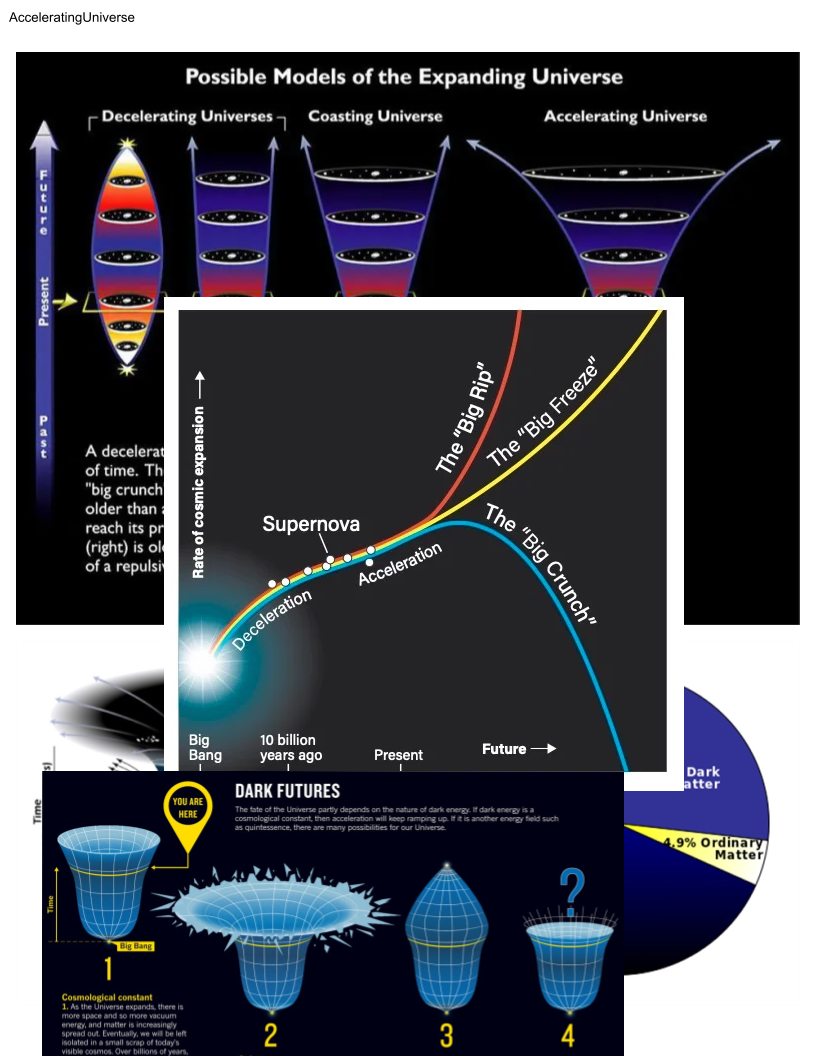
\includegraphics[width=\textwidth,height=\textheight,keepaspectratio]{11_AcceleratingUniverse/accel_illu.png}}
\end{figure}